\documentclass[tikz,border=5]{standalone}
\usepackage{amsmath}
\usepackage{amssymb}
\usepackage[usenames,dvipsnames]{xcolor}
\usepackage[utf8]{inputenc}
\usepackage{tcolorbox}
\usepackage{tikz}
\usetikzlibrary{quantikz}
\usetikzlibrary{calc}
\pgfdeclarelayer{bg}
\pgfsetlayers{bg,main}

\begin{document}

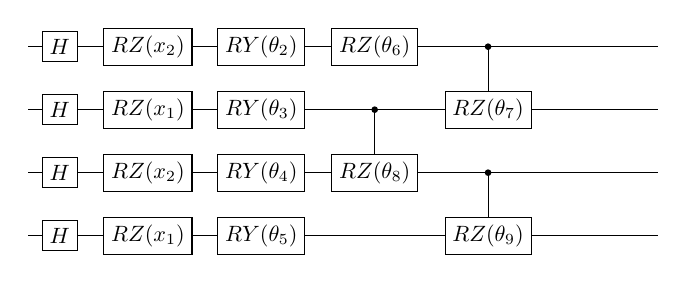
\begin{tikzpicture}[scale=0.8, transform shape]
\begin{scope}
  \node[draw, fill=white] (gate1) at (0.5, -1) {$H$}; %Hadamard
  \node[draw, fill=white] (gate2) at (0.5, -2) {$H$}; %Hadamard
  \node[draw, fill=white] (gate3) at (0.5, -3) {$H$}; %Hadamard
  \node[draw, fill=white] (gate4) at (0.5, -4) {$H$}; %Hadamard
  \node[draw, fill=white] (gate6) at (1.9, -1) {$RZ(x_2)$}; %RZ
  \node[draw, fill=white] (gate7) at (1.9, -2) {$RZ(x_1)$}; %RZ
  \node[draw, fill=white] (gate8) at (1.9, -3) {$RZ(x_2)$}; %RZ
  \node[draw, fill=white] (gate9) at (1.9, -4) {$RZ(x_1)$}; %RZ
  \node[draw, fill=white] (gate11) at (3.7, -1) {$RY(\theta_{2})$}; %RY
  \node[draw, fill=white] (gate12) at (3.7, -2) {$RY(\theta_{3})$}; %RY
  \node[draw, fill=white] (gate13) at (3.7, -3) {$RY(\theta_{4})$}; %RY
  \node[draw, fill=white] (gate14) at (3.7, -4) {$RY(\theta_{5})$}; %RY
  \draw[] (5.5, -1) node[draw, fill=white] (gate15) {$RZ(\theta_{6})$};
  \draw[] (5.5, -2) -- +(0, -1) node[pos=0, circle, fill=black, inner sep=0pt,minimum size=3pt] {{}} node[pos=1, draw, fill=white] (gate16) {$RZ(\theta_{8})$}; %CRZ
  \draw[] (7.3, -1) -- +(0, -1) node[pos=0, circle, fill=black, inner sep=0pt,minimum size=3pt] {{}} node[pos=1, draw, fill=white] (gate17) {$RZ(\theta_{7})$}; %CRZ
  \draw[] (7.3, -3) -- +(0, -1) node[pos=0, circle, fill=black, inner sep=0pt,minimum size=3pt] {{}} node[pos=1, draw, fill=white] (gate18) {$RZ(\theta_{9})$}; %CRZ
\begin{pgfonlayer}{bg}
  \draw (0, -1) -- (10.0, -1);
  \draw (0, -2) -- (10.0, -2);
  \draw (0, -3) -- (10.0, -3);
  \draw (0, -4) -- (10.0, -4);
\end{pgfonlayer}
\end{scope}
\end{tikzpicture}

\end{document}